\chapter{Resultados}
\label{cap:Resultados}

En esta sección se describirá la aplicación del método de trabajo presentado en el Capítulo \ref{cap:Metodologia} en este caso concreto, mostrando los elementos (modelos, diagramas, especificaciones, etc.) más importantes. Este apartado debe explicar cómo la metodología satisface los objetivos planteados en el Capítulo \ref{cap:Objetivo}.

\section{Fase de Inicio}
\label{sec:Resultados.Inicio}

En dicha fase tiene lugar una única iteración, como podemos comprobar en la tabla \ref{tab:iteraciones}. En esta etapa del ciclo de vida del proyecto se llevará a cabo el estudio de viabilidad del mismo, la captura e identificación de los requisitos, y una planificación de sus iteraciones.

\subsection{Estudio de Viabilidad}
\label{subsec:Resultados.Inicio.Viabilidad}

\subsection{Captura de Requisitos}
\label{subsec:Resultados.Inicio.Requisitos}

Tras analizar los objetivos a conseguir descritos en el Capítulo \ref{cap:Objetivo} se analizaron las necesidades y funcionalidades que el sistema debía cumplir, además de considerar las posibles restricciones que afecten al proyecto. Hecho esto, se elaboró la siguiente lista de requisitos funcionales:

\begin{itemize}
    \item \textbf{RF.01 Acceso y/o Registro:}
    El usuario debe poder registrarse en el caso de que lo requiera y, por consiguiente, acceder al resto de funcionalidades del sistema.
    \item \textbf{RF.02 Monitorización del cultivo:}
    El usuario podrá visualizar los datos de su cultivo en tiempo real.
    \item \textbf{RF.03 Gestión de la configuración:}
    El usuario podrá gestionar su cultivo, cambiar sus datos así como los de él mismo.
    \item \textbf{RF.04 Recolección de información:}
    A través de sensores el sistema obtendrá información sobre el terreno.
    \item \textbf{RF.05 Envío de información:}
    Se enviará la información recogida a un servicio a través de la red.
    \item \textbf{RF.06 Análisis y Almacenamiento:}
    La información recogida se analizará para si el riego es o no suficiente en ese instante y se almacenará en una base de datos.
    \item \textbf{RF.07 Envío de acciones:}
    Se enviarán comandos a los dispositivos desplegados en el terreno a aplicar en el volumen de agua suministrado en función de si se ha determinado que el riego es o no suficiente.
    \item \textbf{RF.08 Recepción de comandos:}
    Los dispositivos desplegados en el terreno deben poder recibir los distintos comandos a aplicar a través de la red.
    \item \textbf{RF.09 Aplicación de comandos:}
    Los dispositivos desplegados en el terreno deben poder cambiar, aumentar o disminuir, el volumen de riego aplicado el terreno.
\end{itemize}

También se identificaron los siguientes requisitos no funcionales:

\begin{itemize}
    \item \textbf{RNF.01 Alojamiento en la nube:}
    El servicio en la red al que el usuario accederá debe estar alojado en algún servicio de alojamiento en la nube por la independencia de infraestructura y en libre acceso desde cualquier parte del mundo, además de proporcionar unos sistemas de seguridad básicos.
    \item \textbf{RNF.02 Comunicaciones de largo alcance:}
    Las comunicaciones que se empleen deben ser de largo alcance, ya sean inalámbricas o no, aunque por ello no debe aumentar excesivamente el coste del proyecto.
    \item \textbf{RNF.03 División en secciones:}
    El terreno, al ser una superficie grande, puede subdividirse en zonas más pequeñas para su correcta parametrización en el sistema.
    \item \textbf{RNF.04 Encriptación de mensajes:}
    Todos los datos que se envíen y reciban deben estar encriptados con un algoritmo adecuado para ello para asegurar definitivamente la no manipulación de los mismos.
\end{itemize}

\FloatBarrier
\subsection{Artefactos obtenidos}
\label{subsec:Resultados.Inicio.Artefactos}

Como artefactos resultantes de la finalización de esta fase, con la aplicación del PUD descrito en el Capítulo \ref{cap:Metodologia} y tras la identificación de los requisitos en la Sección \ref{subsec:Resultados.Inicio.Requisitos}, obtenemos una versión inicial del modelo de casos de uso del sistema.

Éstos se han obtenido tras a aplicar la trazabilidad de requisitos a casos de uso con uso del PUD. Partiendo de los requisitos anteriormente especificados, y de la suposición de que varios requisitos funcionales pueden proyectarse en un caso de uso, obtenemos los siguientes casos de uso:

\begin{table}[htb]
    \centering
    \caption{Trazabilidad de requisitos}
    \begin{tabular}[t]{ | r | l |}
        \hline
        \textbf{Caso de Uso} & \textbf{Requisito Funcional} \\ \hline \hline
        CdU.01 Acceso/Registro & RF.01 Acceso y/o Registro \\ \hline
        CdU.02 Visualización & RF.02 Monitorización del cultivo \\ \hline
        CdU.03 Gestión de configuración & RF.03 Gestión de la configuración \\ \hline
        \multirow{2}{*}{CdU.04 Recolección de información}
        & RF.04 Recolección de información \\
        & RF.05 Envío de información \\
        & RF.06 Análisis y Almacenamiento \\
        \hline
        \multirow{2}{*}{CdU.05 Aplicación de comandos}
        & RF.07 Envío de acciones \\
        & RF.08 Recepción de comandos \\
        & RF.09 Aplicación de comandos \\
        \hline
    \end{tabular}
    \label{tab:Trazabilidad.Requisitos}
\end{table}

En la figura \ref{fig:tfg-DCU-00} podemos observar el diagrama de casos de uso del sistema completo a un alto nivel de abstracción.

\begin{figure}[htb]
	\centering
	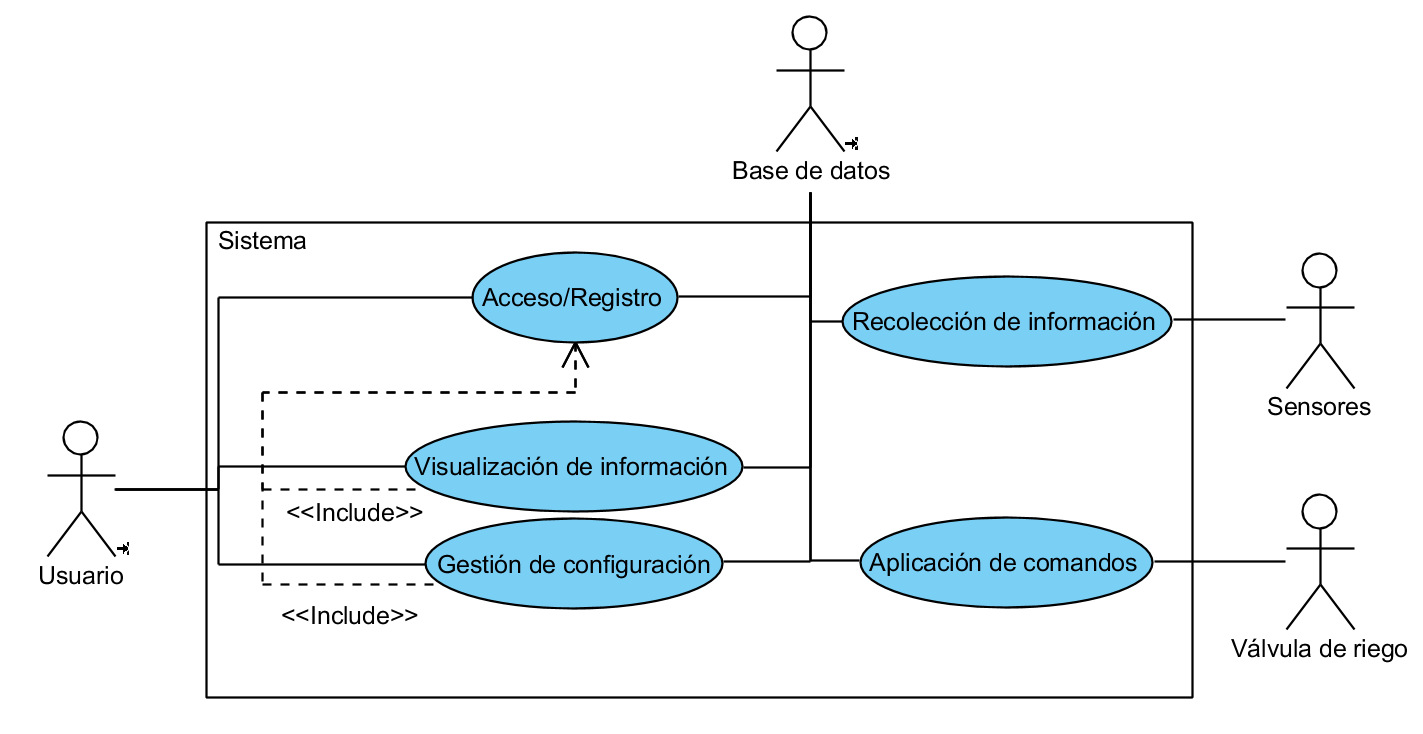
\includegraphics[width=0.80\textwidth]{figs/Modelos/tfg-DCU-00.png}
	\caption[Modelo de Casos de Uso Inicial]{Versión inicial del Modelo de Casos de Uso}
	\label{fig:tfg-DCU-00}
\end{figure}

\FloatBarrier
\subsection{Planificación de Iteraciones}
\label{subsec:Resultados.Inicio.Planificación}

Se ha llevado a cabo una planificación del proyecto con ayuda de la identificación de las distintas iteraciones a completar gracias a la herramienta de Microsoft project.

\begin{table}[hbt]
    \centering
    \caption{Iteración preliminar}
    \label{tab:resultados.planificacion.iter.pre}
    \begin{tabular}[t]{| l || p{8cm} |}
        \hline
        \textbf{Iteración} & Preliminar \\ \hline
        \textbf{Fase} & Inicio \\ \hline
        \multirow{1}{*}{\textbf{Objetivos}}
        & Captura de Requisitos \\ \cline{2-2}
        & Versión inicial del modelo de casos de uso \\ \cline{2-2}
        & Planificación del proyecto \\ \cline{2-2}
        & Estudio de viabilidad \\ \cline{2-2}
        & Anteproyecto aprobado por la comisión académica encargada de dicha tarea \\ \hline
        \multirow{1}{*}{\textbf{Artefactos}}
        & Requisitos funcionales y no funcionales del proyecto \\ \cline{2-2}
        & Diagrama de casos de uso \\ \cline{2-2}
        & Documento del Anteproyecto \\
        \hline
    \end{tabular}
\end{table}

\begin{table}[htb]
    \centering
    \caption{Iteración 1}
    \label{tab:resultados.planificacion.iter.1}
    \begin{tabular}[t]{| l || p{8cm} |}
        \hline
        \textbf{Iteración} & 1 \\ \hline
        \textbf{Fase} & Elaboración \\ \hline
        \multirow{1}{*}{\textbf{Objetivos}}
        & Modelo de casos de uso detallado \\ \cline{2-2}
        & Definición de la línea base de la arquitectura \\ \hline
        \multirow{1}{*}{\textbf{Artefactos}}
        & Segunda versión del diagrama de casos de uso \\ \cline{2-2}
        & Diseño de la arquitectura \\
        \hline
    \end{tabular}
\end{table}

\begin{table}[htb]
    \centering
    \caption{Iteración 2}
    \label{tab:resultados.planificacion.iter.2}
    \begin{tabular}[t]{| l || p{8cm} |}
        \hline
        \textbf{Iteración} & 2 \\ \hline
        \textbf{Fase} & Elaboración \\ \hline
        \multirow{1}{*}{\textbf{Objetivos}}
        & Modelo de análisis \\ \cline{2-2}
        & Modelo de diseño \\ \hline
        \multirow{1}{*}{\textbf{Artefactos}}
        & Diagrama de clases de análisis \\ \cline{2-2}
        & Diagrama de clases de diseño \\
        \hline
    \end{tabular}
\end{table}

\begin{table}[htb]
    \centering
    \caption{Iteración 3}
    \label{tab:resultados.planificacion.iter.3}
    \begin{tabular}[t]{| l || p{8cm} |}
        \hline
        \textbf{Iteración} & 3 \\ \hline
        \textbf{Fase} & Construcción \\ \hline
        \multirow{1}{*}{\textbf{Objetivos}}
        & Implementación del caso de uso CdU.01 \\ \cline{2-2}
        & Pruebas de integración \\ \hline
        \multirow{1}{*}{\textbf{Artefactos}}
        & Diagrama de secuencia del caso de uso CdU.01 \\ \cline{2-2}
        & Resultado de las pruebas \\
        \hline
    \end{tabular}
\end{table}

\begin{table}[htb]
    \centering
    \caption{Iteración 4}
    \label{tab:resultados.planificacion.iter.4}
    \begin{tabular}[t]{| l || p{8cm} |}
        \hline
        \textbf{Iteración} & 4 \\ \hline
        \textbf{Fase} & Construcción \\ \hline
        \multirow{1}{*}{\textbf{Objetivos}}
        & Implementación del caso de uso CdU.02 \\ \cline{2-2}
        & Pruebas de integración \\ \hline
        \multirow{1}{*}{\textbf{Artefactos}}
        & Diagrama de secuencia del caso de uso CdU.02 \\ \cline{2-2}
        & Resultado de las pruebas \\
        \hline
    \end{tabular}
\end{table}

\begin{table}[htb]
    \centering
    \caption{Iteración 5}
    \label{tab:resultados.planificacion.iter.5}
    \begin{tabular}[t]{| l || p{8cm} |}
        \hline
        \textbf{Iteración} & 5 \\ \hline
        \textbf{Fase} & Construcción \\ \hline
        \multirow{1}{*}{\textbf{Objetivos}}
        & Implementación del caso de uso CdU.03 \\ \cline{2-2}
        & Pruebas de integración \\ \hline
        \multirow{1}{*}{\textbf{Artefactos}}
        & Diagrama de secuencia del caso de uso CdU.03 \\ \cline{2-2}
        & Resultado de las pruebas \\
        \hline
    \end{tabular}
\end{table}

\begin{table}[htb]
    \centering
    \caption{Iteración 6}
    \label{tab:resultados.planificacion.iter.6}
    \begin{tabular}[t]{| l || p{8cm} |}
        \hline
        \textbf{Iteración} & 6 \\ \hline
        \textbf{Fase} & Construcción \\ \hline
        \multirow{1}{*}{\textbf{Objetivos}}
        & Implementación del caso de uso CdU.04 \\ \cline{2-2}
        & Pruebas de integración \\ \hline
        \multirow{1}{*}{\textbf{Artefactos}}
        & Diagrama de secuencia del caso de uso CdU.04 \\ \cline{2-2}
        & Resultado de las pruebas \\
        \hline
    \end{tabular}
\end{table}

\begin{table}[htb]
    \centering
    \caption{Iteración 7}
    \label{tab:resultados.planificacion.iter.7}
    \begin{tabular}[t]{| l || p{8cm} |}
        \hline
        \textbf{Iteración} & 7 \\ \hline
        \textbf{Fase} & Construcción \\ \hline
        \multirow{1}{*}{\textbf{Objetivos}}
        & Implementación del caso de uso CdU.05 \\ \cline{2-2}
        & Pruebas de integración \\ \hline
        \multirow{1}{*}{\textbf{Artefactos}}
        & Diagrama de secuencia del caso de uso CdU.05 \\ \cline{2-2}
        & Resultado de las pruebas \\
        \hline
    \end{tabular}
\end{table}

\begin{table}[htb]
    \centering
    \caption{Iteración 8}
    \label{tab:resultados.planificacion.iter.8}
    \begin{tabular}[t]{| l || p{8cm} |}
        \hline
        \textbf{Iteración} & 8 \\ \hline
        \textbf{Fase} & Transición \\ \hline
        \multirow{1}{*}{\textbf{Objetivos}}
        & Despliegue del sistema completo \\ \hline
        \multirow{1}{*}{\textbf{Artefactos}}
        & Sistema desplegado y funcional \\
        \hline
    \end{tabular}
\end{table}

\begin{table}[htb]
    \centering
    \caption{Iteración 9}
    \label{tab:resultados.planificacion.iter.9}
    \begin{tabular}[t]{| l || p{8cm} |}
        \hline
        \textbf{Iteración} & 9 \\ \hline
        \textbf{Fase} & Transición \\ \hline
        \multirow{1}{*}{\textbf{Objetivos}}
        & Realización de pruebas en el sistema desplegado \\ \hline
        \multirow{1}{*}{\textbf{Artefactos}}
        & Resultados de las pruebas \\
        \hline
    \end{tabular}
\end{table}

\begin{table}[htb]
    \centering
    \caption{Iteración 10}
    \label{tab:resultados.planificacion.iter.10}
    \begin{tabular}[t]{| l || p{8cm} |}
        \hline
        \textbf{Iteración} & 10 \\ \hline
        \textbf{Fase} & Transición \\ \hline
        \multirow{1}{*}{\textbf{Objetivos}}
        & Documentación del proyecto \\ \cline{2-2}
        & Elaboración de los manuales de usuario correspondientes \\ \hline
        \multirow{1}{*}{\textbf{Artefactos}}
        & Memoria del TFG \\ \cline{2-2}
        & Manual de usuario \\ \hline
        \hline
    \end{tabular}
\end{table}